\chapter{Introducción}
\graphicspath{{./figs/01_intro/}}
\chapterquote{La destrucción es obra de una tarde. La creación es obra de una vida.}{Kamahl, acólito druida}
\section{Motivación}\label{S:motivacion}
Dentro de la multitud de materiales existentes, los sólidos cristalinos son aquellos que tienen más impacto en el desarrollo de nuestra vida cotidiana. 
Los sólidos cristalinos son materiales que están constituidos por cristales, que son arreglos periódicos de átomos. 
Dado que en el transcurso de este trabajo sólo se hablará de sólidos cristalinos, cuando se hable de sólido, material o muestra, siempre se sobreentenderá que se está hablando de un sólido cristalino.

\begin{figure}[h!]
  \centering
  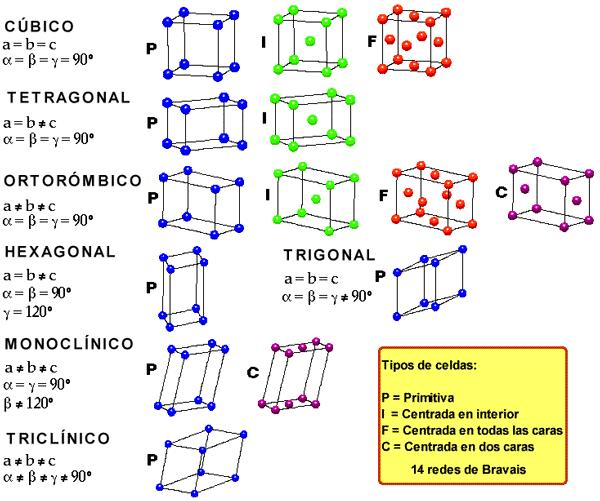
\includegraphics[width=0.6\textwidth]{Bravais}
  \caption{Las 14 Redes de Bravais posibles para un material tridimensional.}
  \label{fig:Bravais}
\end{figure}

La unidad básica de un cristal es la denominada celda unidad, que se repite en las tres dimensiones del espacio, dándole al cristal una simetría de traslación. Utilizando los métodos de la teoría de grupos, se puede demostrar que existen sólo 14 formas de llenar el espacio con arreglos periódicos de átomos (Fig. \ref{fig:Bravais}), es decir, existen 14 tipos diferentes de celdas unitarias, que se denominan redes de Bravais\cite{hahn2005international}.

Sin embargo, a pesar de la variedad de posibles arreglos atómicos disponibles, se observa que en la naturaleza los metales tienden a formar sólo tres de esas estructuras, que se muestran en la Fig. \ref{fig:celdasmetalicas} y que se denominan Cúbica Centrada en las Caras (FCC), Cúbica Centrada en el Cuerpo (BCC) y Hexagonal Compacta (HCP). 
Las siglas que se usarán para caracterizar a cada una de estas celdas están basadas en la nomenclatura inglesa, \textit{Face Centered Cubic}, \textit{Body Centered Cubic} y \textit{Hexagonal Close Packed}. En este trabajo se trabajará con materiales metálicos que tienen alguna de estas tres simetrías, y se pondrá especial foco en los materiales FCC y BCC.

\begin{figure}[h!]
  \centering
  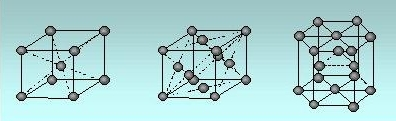
\includegraphics[width=0.5\textwidth]{celdasmetalicas}
  \caption{Las tres redes de Bravais que se ibservan en los materiales metálicos.}
  \label{fig:celdasmetalicas}
\end{figure} 

Según el principio de Neumann\cite{nye1985physical}, las propiedades básicas de un sólido cristalino están determinadas en primer lugar por la de la celda unidad, y serán en general anisotrópicas, es decir dependerán de la orientación de dicha celda respecto a un cierto sistema de referencia.
En un dado sólido, puede ocurrir que todos sus cristales tengan la misma orientación, en cuyo caso se dice que ese material es un monocristal.
Si por el contrario, el sólido está constituido por cristales orientados en cualquier dirección, y todas las orientaciones se encuentran igualmente representadas, se dice entonces que el material es un policristal.
En este caso, las propiedades macroscópicas del cristal se pueden obtener a partir de promediar las propiedades de la celda unidad en todas las orientaciones posibles.
El caso más general consistirá en una situación intermedia entre un monocristal y un policristal, es decir, los cristales tendrán una o más orientaciones preferenciales y habrá una cierta distribución alrededor de dichas orientaciones, lo que constituirá la textura de dicho material. 
La textura de un material es el segundo factor que condicionará la anisotropía de las propiedades macroscópicas de un sólido cristalino.

La relación entre textura, propiedades mecánicas y procesos de fabricación es de gran interés puro, pero especialmente aplicado, ya que la capacidad de controlar la textura, y con ello la anisotropía de las propiedades mecánicas de los materiales, puede implicar beneficios económicos importantes.
Uno de los ejemplos más estereotípicos que se suele citar es el ``orejeado'' que puede producirse durante el embutido de chapas metálicas (Fig. \ref{fig:earing}), donde la anisotropía causada por la textura puede resultar en que la copa no tenga una altura homogénea, lo que produce un exceso importante en la chatarra que produce al cortar la boca de esas copas para eliminar el orejeado.

\begin{figure}[h!]
  \centering
  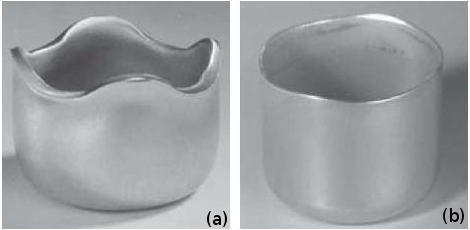
\includegraphics[width=0.5\textwidth]{earingxcf}
  \caption{Ejemplo de la influencia de la influencia de la textura en la respuesta mecánica que se puede observar en un material metálico, aluminio en este caso. La figura (a) muestra un ejemplo típico de ``orejeado'', producto de una anisotropía producida por la textura. El material de la figura (b) tiene una textura que resulta en una respuesta más isotrópica del material ante el embutido, eliminando así el orejeado. }
  \label{fig:earing}
\end{figure}

Adicionalmente la textura no sólo condiciona las propiedades mecánicas de los materiales, sino que también influencia cómo estos materiales acumularán defectos una vez sometidos a diferentes solicitaciones. 
Por ejemplo, más adelante en esta tesis se verá como al laminar el acero, se favorecen dos tipos de orientaciones, pero los defectos tienden a acumularse en sólo una de ellas, lo cual a su vez afecta otras propiedades del acero como ser su dureza, ductilidad, etc.

A partir de estas motivaciones surge este trabajo, en donde se propone estudiar la anisotropía de distintas aleaciones metálicas, así como buscar relaciones entre las deformaciones mecánicas sufridas por las muestras, su textura y los defectos acumulados en las mismas.

\section{Cristalografía de Rayos X}\label{S:DRX}
Los rayos X son una herramienta de vital importancia para el estudio de los materiales cristalinos, ya que de la interacción entre ambos se pueden observar los detalles acerca del ordenamiento de los átomos en un dado material.

Para entender los principios importantes de la cristalografía de rayos X, se parte de un haz monocromático de radiación X de longitud de onda $\lambda$ y vector de onda $\mathbf{k_i}$ que incide sobre una dada muestra cristalina formando un ángulo $\theta$ con la familia de planos cristalinos $\{hkl\}$, como se observa en la Fig. \ref{fig:Bragg}.

\begin{figure}[htb!]
  \centering
  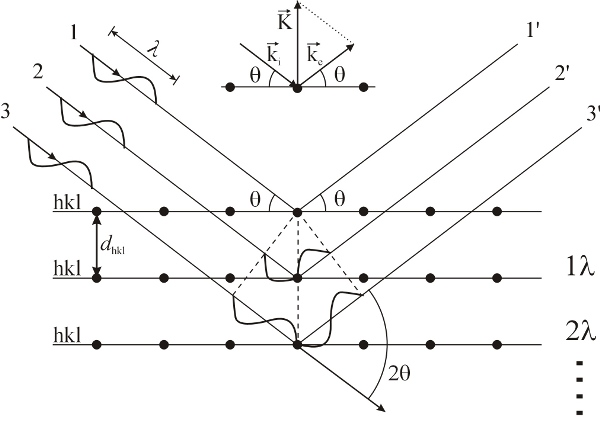
\includegraphics[width=\imsize]{BraggLaw}
  \caption{Ley de Bragg}
  \label{fig:Bragg}
\end{figure}

Si el haz interactúa con la muestra elásticamente, será dispersado con la misma longitud de onda inicial, pero en una dirección marcada por el vector de onda $\mathbf{k_e}$, que cumplirá $\lvert \mathbf{k_i} \rvert \ = \ \lvert \mathbf{k_e} \rvert \ = \ \frac{2\pi}{\lambda}$, y que formará el mismo ángulo con la familia de planos $\{hkl\}$.
Si el cristal es infinito y está libre de cualquier tipo de distorsiones, habrá interferencia constructiva del haz dispersado sólo cuando el vector de dispersión $\mathbf{K}$ es igual a un vector de la red recíproca correspondiente a la familia de planos $\{hkl\}$:
\begin{equation}
  \mathbf{K} \ = \ \mathbf{k_e} - \mathbf{k_i} \ = \ \mathbf{G_{hkl}}
  \label{eq:Braggvec}
\end{equation}
\noindent
siendo $\mathbf{G_{hkl}}$ el vector de la red recíproca que corresponde a la familia de planos $\{hkl\}$.
Ahora bien, como se puede ver en la Fig \ref{fig:Bragg}, $\displaystyle \lvert \mathbf{K} \rvert = \frac{2\sin\theta_B}{\lambda}$, y como $\displaystyle\lvert \mathbf{G_{hkl}} \rvert = \frac{n}{d_{hkl}}$, la condición de Bragg \ref{eq:Braggvec} puede escribirse también como:
\begin{equation}
  2 \ d_{hkl} \ \sin(\theta_{B}) \ = \ n \ \lambda
  \label{eq:Bragg}
\end{equation}
\noindent
siendo $d_{hkl}$ la distancia interplanar de la familia de planos $\{hkl\}$, 2$\theta_{B}$ el ángulo formado entre el haz incidente y el haz reflejado cuando se cumple la condición de Bragg y $n$ el número de orden de difracción. La Ec. \ref{eq:Bragg}, se llama Ley de Bragg y es la ecuación fundamental de la difracción de Rayos X (XRD). 

La Ley de Bragg es válida en la medida que se cumplan la condiciones de dispersión cinemática y la condición de difracción de Fraunhoffer. 
La primer condición se cumple cuando el fotón de rayos X que es dispersado interactúa solamente con un átomo de la muestra, y no es válida cuando se tiene un cristal verdaderamente perfecto.
Por otro lado, la condición de Fraunhoffer implica que el detector se encuentra a una distancia mucho mayor que la longitud característica del cristal que está dispersando la radiación.
Para las configuraciones de laboratorio típicas, esto implica que no se pueden estudiar cristales con dimensiones mayores a $\sim 1\,\mu m$.
Ambas aproximaciones serán válidas para los materiales y las condiciones experimentales mencionadas en este trabajo.

\nomenclature{$\lambda$}{Longitud de onda}
\nomenclature{$d_{hkl}$}{Distancia interplanar para la familia de planos $hkl$}
\nomenclature{$\theta_B$}{Ángulo de Bragg}
\nomenclature{XRD}{Difracción de Rayos X}
\nomenclature{$\mathbf{k_i}$}{Vector de onda de la radiación incidente.}
\nomenclature{$\mathbf{k_e}$}{Vector de onda de la radiación saliente.}
\nomenclature{$\mathbf{K}$}{Vector diferencia entre los vectores de onda de las radiaciones incidente y saliente. También llamado vector de dispersión.}
\nomenclature{$\mathbf{G}$}{Vector de la red recíproca.}
\nomenclature{$\mathbf{K_B}$}{Vector de dispersión que cumple la ley de Bragg.}


Una consecuencia de la ley expresada en la Ec. \ref{eq:Bragg} es que para un cierto haz incidente habrá reflexiones cuyas distribución de intensidades serán funciones deltas de Dirac, con intensidad infinita para el ángulo $\theta_{B}$ e intensidad nula para los ángulos $\theta$ que no cumplan con la condición de Bragg. 
Como resultado, los ``picos'' de difracción tendrán un ancho nulo. 
Si, como ocurre en la práctica, el número de planos que contribuyen a la reflexión es finito, la distribución angular de intensidades tendrán un ancho y altura finitos, y lo mismo ocurrirá si la red de átomos tiene distorsiones, es decir, si los átomos no se encuentran en un arreglo perfectamente periódico.

En un experimento de XRD real aparecerán además otras contribuciones que ensancharán los picos de difracción. 
Por ejemplo, el haz incidente no será puntual ni estará constituido por haces completamente paralelos, sino que tendrá un tamaño finito y estará comprendido entre haces que tendrán cierta divergencia angular.
Además, el haz no será completamente monocromático, sino que estará integrado por rayos X con longitudes de onda en un intervalo $(\lambda \ \pm \ \Delta \lambda)$.
Todos estos factores contribuirán a que haya haces difractados en las vecindades de $\theta_{B}$, aumentando el ancho de los picos de difracción. 
Una parte importante de esta tesis se tratará de obtener información acerca de la microestructura de los materiales a partir del ensanchamiento de los picos de difracción, por lo que la correcta clasificación y cuantificación de los efectos instrumentales será motivo de discusión permanente en los capítulos siguientes.

\subsection{Estudios de ancho de pico: Revisión bibliográfica y estado del arte}\label{SS:XRD-LPA} 
Si no se tienen en cuenta los diferentes efectos instrumentales se puede afirmar que, a partir del estudio del ensanchamiento y la forma de los perfiles de intensidad de los picos medidos en un experimento de XRD, es posible obtener información microestructural del material, como la cantidad y tipo de defectos presentes, o la distribución de tamaño de los dominios coherentes de difracción (cristalitas).
Al conjunto de técnicas y métodos del campo de la cristalografía que utilizados para obtener este tipo de información se los conoce como Estudios de Ancho de Pico, o LPA, por sus siglas en inglés (\textit{Line Profile Analysis}).
Aunque el término LPA fue acuñado muchos años después, la técnica, aunque rudimentaria, es tan antigua como los primeros experimentos de XRD, y fue implementada independientemente por Hull en Estados Unidos y Debye y Scherrer en Alemania. 
Mientras investigaba el tamaño de partículas de oro y plata en sistemas coloidales, Scherrer incluyó la ecuación que luego llevaría su nombre\cite{Scherrer1918}:

\begin{equation}
  H \ = \ 2 \sqrt{\frac{\ln(2)}{\pi}} \ \frac{\lambda}{L \ \cos(\theta_B)}
  \label{eq:Scherrer}
\end{equation}
\noindent
Donde $H$ denota el ancho del pico a la mitad de su intensidad máxima (también abreviado FWHM), $L$ es la longitud característica de la cristalita en la dirección perpendicular a la familia de planos $\{hkl\}$ y el factor numérico $2\sqrt{\ln(2)/\pi}$ se usa para convertir $H$ al ancho integral del pico, suponiendo que el mismo tiene forma Gaussiana.
Los trabajos que siguieron se dedicaron a mejorar las estimaciones de tamaño y forma de las cristalitas, así como estudiar los perfiles de picos a partir de funciones Lorentzianas y mezclas de funciones Lorentzianas y Gaussianas.
En el año 1938 Jones\cite{Jones16} señaló que el perfil de intensidades medido en un experimento de XRD, $I_{exp}$, es la convolución del perfil $I_{muestra}$ que se obtendría de la muestra y el debido a todos los efectos instrumentales, $I_{inst}$, es decir:
\begin{equation}
  I_{exp} \ = \ I_{muestra} \ \otimes \ I_{inst}
  \label{eq:conv}
\end{equation}
\noindent
De esta manera, Jones logró remover las contribuciones de las líneas $K\alpha_2$ de la radiación del cobre en las mediciones de tamaño de cristalita.
En el año 1949 Hall\cite{WHHall1949} usó la formulación de Stokes y Wilson para proponer un método para separar las contribuciones de los efectos de tamaño de cristalita y de deformación de la red cristalina, basándose en el hecho de que cada contribución tiene una variación característica con el orden de difracción $\{hkl\}$.
Al graficar el ancho integral de cada pico de difracción en función de $K$, los puntos se acomodan en una recta cuya pendiente está relacionada con el nivel de deformación de la red, y cuya ordenada al origen es el recíproco del tamaño de cristalita promedio ($D$):
\begin{equation}
  \Delta K \ = \  \beta \ \cos\left(\frac{\theta}{\lambda}\right) \ = \frac{1}{D} \ + \ 2 \ \epsilon \ K
  \label{eq:WHPlot}
\end{equation}
\noindent
siendo $\epsilon$ una cantidad que es proporcional a la distorsión de la red cristalina y $\beta$ es el ancho integral de cada reflexión.
La primera versión del método de Williamson-Hall, que es como se llamó a la aplicación de la Ec. \ref{eq:WHPlot}, se basa en la suposición de que los picos de difracción tienen un perfil lorentziano.
Si los perfiles tienen un carácter gaussiano, muchos pasos en la deducción son iguales, pero el resultado final es lo que se denomina la forma cuadrática de la ecuación de Williamson-Hall\cite{Scardi2004}:
 \begin{equation}
  (\Delta K)^2 \ = \ \left[\beta \ \cos\left(\frac{\theta}{\lambda}\right)\right]^2 \ = \left(\frac{1}{D}\right)^2 \ + \ 4 \ \epsilon^2 \ K^2
  \label{eq:WHPlot2}
\end{equation}
\noindent
Conceptualmente, lo que dicen las Ecs. \ref{eq:WHPlot} y \ref{eq:WHPlot2} es que el ensanchamiento producido por el tamaño finito de cristalita es independiente del orden de difracción $hkl$ o el vector de difracción $K$, mientras que la contribución debida a las  distorsiones de la red cristalina crecen linealmente o cuadráticamente, respectivamente, con el vector $K$.

En el año 1949, Warren y Averbach\cite{WarrenAverbach1949} también utilizaron la formulación de Stokes y Wilson para derivar otro método para separar las contribuciones de distorsión y tamaño al ensanchamiento de los picos de rayos X. 
El método de Warren-Averbach se basa en el hecho de que la transformada de Fourier de la convolución de dos funciones es simplemente el producto de las transformadas de Fourier de dichas funciones, y como el perfil de intensidades $I_{muestra}$ es la convolución del perfil obtenido por las contribuciones de tamaño $I_{T}$ y distorsión $I_{D}$, los coeficientes de Fourier del perfil de línea de la muestra $A_n$ son el producto de los coeficientes de tamaño $A_n^T$ y distorsión $A_n^D$:
\begin{equation}
  A_n \ = \ A_n^T \ A_n^D
  \label{eq:FCoeff}
 \end{equation}
\noindent
En este caso, si se supone que las cristalitas son de forma esférica y que su distribución de tamaño de tipo lognormal\cite{WikiLognormal} y se supone un perfil de deformación de tipo gaussiano, se puede llegar a la ecuación que se emplea cuando se aplica el método de Warren-Averbach:
\begin{equation}
  \ln(A_n(l)) \ = \ \ln(A_n^T) \ - \ 2 \pi^2 n^2 l^2 \ <e^2>
  \label{eq:WAPlot}
 \end{equation}
\noindent
En la Ec. \ref{eq:WAPlot}, $l$ es el orden de una dada reflexión, $<e^2>$ es la deformación cuadrática media de la red cristalina y el resto de los símbolos son los definidos anteriormente.

\nomenclature{$H$ o $FWHM$}{Ancho de pico a media altura. También abreviado como FWHM por sus siglas en inglés (Full Witdth at Half Maximum).}
\nomenclature{$<e^2>$}{Deformación cuadrática media de la red cristalina}
\nomenclature{$L$}{Orden de reflexión. Mentira. Escribirlo bien.}
\nomenclature{$A_n$}{n-ésimo coeficiente de Fourier}

Una limitación importante de los métodos de Williamson-Hall (WH) y de Warren-Averbach (WA) es que no toman en cuenta la anisotropía en la deformación de la red cristalina. 
Matemáticamente, eso significa que los términos de deformación en las Ecs. \ref{eq:WHPlot}, \ref{eq:WHPlot2} y \ref{eq:WAPlot} son funciones monótonas de $K$ y $l$, respectivamente.
En la práctica, si en el material estudiado las dislocaciones son un mecanismo de deformación importante, se observará que el ensanchamiento $\Delta K$ no es una función monótona de $K$ sino que existe cierta dispersión, como se ve en la Fig \ref{fig:MWH}-(a). 

\begin{figure}[!htb]
  \centering
  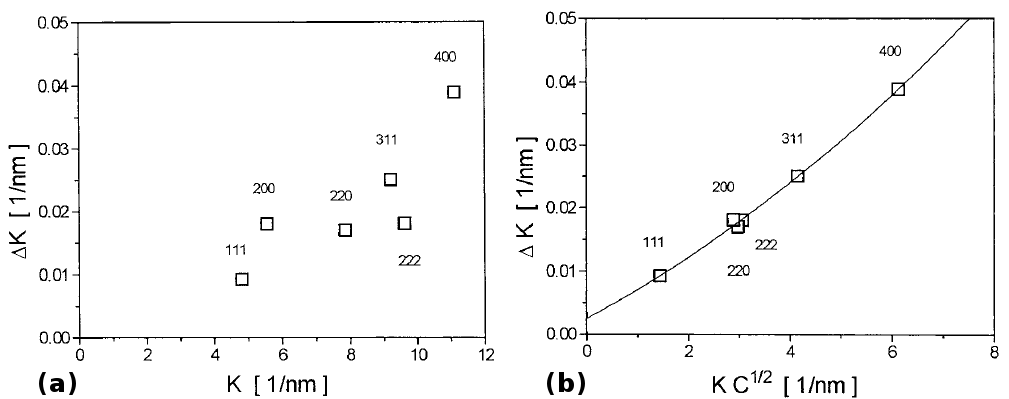
\includegraphics[width=\textwidth]{MWH}
  \caption{Ejemplo del ensanchamiento anisotrópica. Imágenes obtenidas de \cite{Ungar1999}}
  \label{fig:MWH}
\end{figure}

En ensanchamiento anisotrópico puede tener multitud de causas, entre ellas:
\begin{enumerate}[(i)]
  \item Errores sistemáticos y estadísticos en la medición. 
  \item Anisotropía en el tamaño de cristalita.
  \item Las cristalitas que contribuyen al ensanchamiento de cada pico tienen distinta densidad de dislocaciones.
  \item El campo de deformaciones en el medio elástico es anisótropo, con lo cual la contribución al ensanchamiento de los picos de difracción será diferente para cada familia de planos $\{hkl\}$.
  \item Existen defectos de tipo planar que contribuyen al ensanchamiento de los picos de difracción.
\end{enumerate}

La causa (i) sólo se puede minimizar a través de una cuidadosa planificación y ejecución de los experimentos, aunque siempre va a estar presente en alguna medida, y va a tener mayor importancia cuando se esté estudiando el perfil de picos de baja intensidad respecto al ruido de fondo. 
La causa (ii) es difícil de saber a priori y va a depender fuertemente de la historia de la muestra. 
La causa (iii) está fuertemente relacionada con la textura del material, sus características cristalográficas y el tipo de procesos a las que fue sometida. 
La causa (iv) siempre estará presente y también será dificil de determinar a priori, salvo para casos particulares.
Finalmente la causa (v) podrá visualizarse en ciertos casos estudiando la asimetría de los picos de difracción, así como estudiando la dependendencia de la anisotropía con el orden de difracción $\{hkl\}$ y estudiando el corrimiento de los picos de difracción.

Las formulaciones del método de WH y de WA involucran ciertas suposiciones implicitas para resolver los problemas planteados, a saber, que todas las cristalitas tienen forma esférica y que tienen el mismo tamaño, que no hay defectos planares y que la deformación causada por las dislocaciones es isótropa. 

Hacia finales de los '90 y principios de los 2000 Ungar et al modificaron la formulación de WH y WA para tomar en cuenta la anisotropía en el campo de deformaciones de la red cristalina a través del concepto de los factores de contraste.

\begin{figure}[!htb]
  \centering
  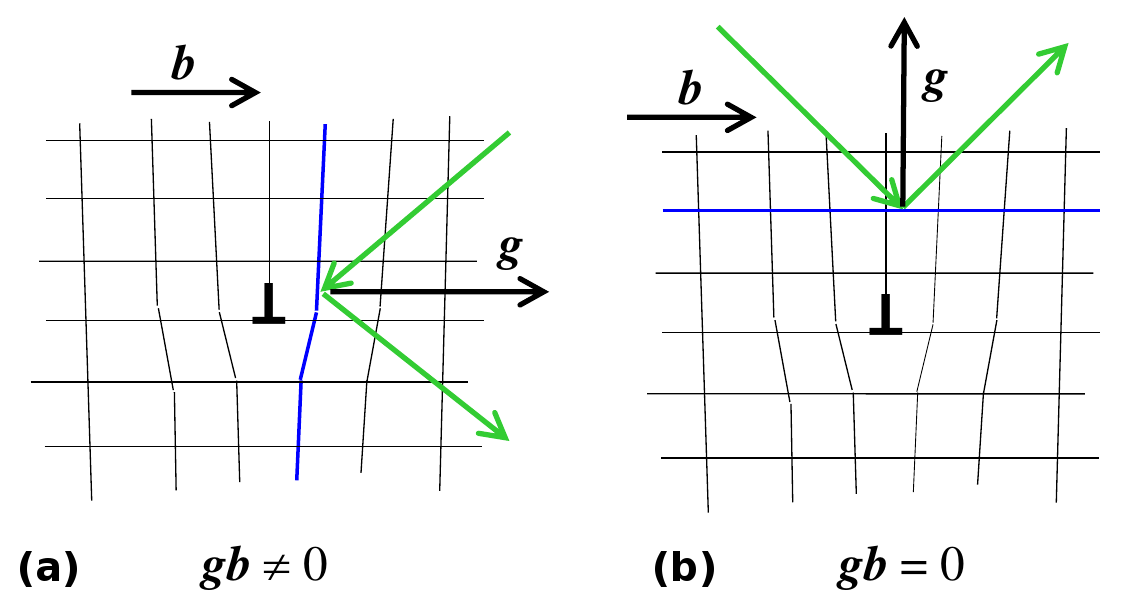
\includegraphics[width=0.8\textwidth]{Contrast}
  \caption{Ejemplo de la influencia del factor de contraste para dos casos extremos. Ver si puedo encontrar una referencia.}
  \label{fig:contrast}
\end{figure}

El modelo del factor de contraste toma en cuenta que las dislocaciones no son igualmente visibles para cualquier plano cristalino, es decir, la contribución de una dada dislocación al ancho de un determinado pico de difracción definido por el vector $\mathbf{G_{hkl}}$ va a depender de la orientación relativa entre $\mathbf{G_{hkl}}$ y el vector de burgers $\mathbf{b}$ de esa dislocación, tal como se muestra la Fig. \ref{fig:contrast} para los dos casos extremos que pueden ocurrir al estudiar para una dislocación de borde en una red cúbica.

Tanto en la parte (a) de la figura como en la (b) se tiene una dislocación de borde cuyo vector de burgers tiene una dirección horizontal con sentido hacia la derecha. 
Ahora bien, si en un experimento de difracción se observan los planos verticales, es decir se tiene $\mathbf{g} \ \parallel \ \mathbf{b}$, la contribución de esa dislocación hacia el ensanchamiento de pico será máxima, y esto se correlaciona con el hecho que que la distorsión que la dislocación ocasiona en la red cristalina es más visible.
Por otro lado, al observar los planos horizontales se tiene $\mathbf{g} \ \perp \ \mathbf{b}$ y la contribución de esa dislocación al ensanchamiento de ese pico será nula, o muy pequeña.
Notar que al ver los planos horizontales la deformación producida en la red cristalina es mucho menos visible.

Este ejemplo muestra que se puede pensar en el factor de contraste $C$ como una cantidad que va a corregir el hecho de que una dada dislocación es más o menos ``visible'' en un experimento de difracción, dependiendo del plano cristalino analizado.
La correcta determinación de estos factores es fundamental si se quiere hacer una cuantificación adecuada de la densidad de dislocaciones de un material.
Como regla general, el factor de contraste será una cantidad que depende tanto del vector de difracción $\mathbf{G}$ como del tipo de dislocación presente en el material, así como de las constantes elásticas del material mismo:
\begin{equation}
  C \ = \ C(\mathbf{G},\mathbf{b},\mathbf{l},c_{ij})
  \label{eq:contrast}
\end{equation}
\noindent
Donde $\mathbf{G}$ y $\mathbf{b}$ son las cantidades definidas previamente, $\mathbf{l}$ es el vector de línea de la dislocación y $c_{ij}$ representan las componentes del tensor de elasticidad del material.
El cálculo de $C$ a partir de la Ec. \ref{eq:contrast} para un material elásticamente anisotróopico es una tarea que, además de laboriosa, requiere conocer a priori el tipo de dislocaciones presentes en el material y los sistemas de deslizamiento activos, lo que en general no ocurre.
Para sistemas cristalinos cúbicos y hexagonales Ungár et al\cite{Dragomir1999,Dragomir2002} han encontrado expresiones analíticas para calcular el factor de contraste de cualquier tipo de dislocación, siempre que se sepa el sistema de deslizamiento activo y el tipo de dislocación presente. En particular, para sistemas cúbicos se tiene que la Ec. \ref{eq:contrast} toma una forma sencilla:

\begin{equation}
  C \ = \ C(hkl) \ = \ A \ + \ B \ H^2
  \label{eq:contrast2}
\end{equation}
\noindent
con
\begin{equation}
  H^2 \ = \ \frac{h^2k^2 \ + \ h^2l^2 \ + \ k^2l^2}{(h^2 \ + \ k^2 \ + \ l^2)^2}
  \label{eq:H2}
\end{equation}
\noindent
un invariante de cuarto orden de los índices de Miller $hkl$, y $A$ y $B$ constantes que pueden calcularse a para dislocaciones de hélice y borde a partir de las constantes elásticas del material.
Si se observa con detenimiento la Ec. \ref{eq:H2} se puede notar que $C(h00) \ = \ A$, por que la Ec. \ref{eq:contrast2} suele escribirse de la forma:
\begin{equation}
  C(hkl) = C_{h00}\ (1 \ - \ q\ H^2)
  \label{eq:contrast3}
\end{equation}
\noindent
donde $A \ = \ C_{h00}$ y $q \ = \ -B/A$ es un factor que puede relacionarse con el carácter hélice/borde de las dislocaciones presentes.
Vale notar que la Ec. \ref{eq:contrast3} es válida sólo si $C_{h00} \neq 0$, cosa que no ocurre en todos los casos, aunque sí lo suficiente como para darle a la Eq. \ref{eq:contrast3} una generalidad aceptable.
\nomenclature{$C$}{Factor de contraste de una dislocación.}
\nomenclature{$\bar{C}$}{Factor de contraste promedio.}
\nomenclature{$H^2$}{Invariante de cuarto orden que determina el factor de contraste promedio.}
\nomenclature{$\bar{C}_{h00}$}{Factor de contraste promedio para los planos {h00}}
\nomenclature{$q$}{Carácter hélice-borde de una dislocación}
\nomenclature{$\mathbf{b}$}{Vector de burgers de una dislocación.}
\nomenclature{$\mathbf{l}$}{Vector de línea de una dislocación.}
\nomenclature{$c_{ij}$}{Constantes elásticas de un material.}

A partir de la implementación del método de los factores de contraste, se puede avanzar en relacionar la deformación cuadrática media de la red cristalina $<e^2>$ con la densidad de dislocaciones. En particular, si la principal causa de deformación de la red cristalina son dislocaciones, la deformación cuadrática media puede escribirse\cite{Wilkens1970}:
\begin{equation}
  <e^2> \ = \ \frac{\rho \ C \ b^2}{4 \pi} \ f\left(\frac{l}{R_e}\right) \ \xrightarrow[l \to 0]{} \ - \ \frac{\rho \ C \ b^2}{4 \pi} \ln \left(\frac{l}{R_e}\right)
  \label{eq:Wilkens}
\end{equation}
\noindent
donde $b$ es la longitud del vector de burgers de las dislocaciones, $C$ es el factor de contraste definido en \ref{eq:contrast} y \ref{eq:contrast3}, $\rho$ es la densidad de dislocaciones del material y $R_e$ es el radio de corte del campo de deformación producido por las dislocaciones y $f$ es la función de Wilkens. 
Cuando se busca analizar los detalles de la microestructura, $R_e$ suele reemplazarse por el factor de Wilkens $M \ = \ R_e\,\sqrt{\rho}$, que da una idea no sólo de la cantidad de dislocaciones, sino de cómo éstas interactúan entre si para deformar la estructura cristalina. Se pueden distinguir tres casos:

\begin{itemize}
  \item[$\bullet$] Si $M \ = \ 1 $ En este caso $R_e\,=\,\frac{1}{\sqrt{\rho}}$ y la longitud del campo de deformación producido por las dislocaciones es igual a la distancia promedio entre las mismas.
  \item[$\bullet$] Si $M \ << \ 1 $ el campo de deformaciones producido por las dislocaciones es menor que la distancia promedio entre ellas y es apantallado por un arreglo de dislocaciones correlacionadas que forman dipolos. En este caso el perfil de ensanchamiento resultante tiende a tener una forma lorentziana.
  \item[$\bullet$] Por otro lado si $M \ >> \ 1 $ las dislocaciones están distribuidas aleatoriamente, no interactúan entre ellas y el campo de deformaciones es de largo alcance. El perfil resultante de esta microestructura tiene un aspecto gaussiano.
\end{itemize}

Un análisis más detallado de la contribución de las dislocaciones al ensanchamiento de picos de difracción revela que la Ec. \ref{eq:Wilkens} es el primer orden de un desarrollo más complejo\cite{Groma1988}:
\begin{equation}
  \begin{split}
      <e^2> \ = & \ - \ \frac{Cb^2}{4 \pi}\left< \rho \right> \ln \left( l/R_e \right) \ \\
     & \ +  \ \frac{1}{4\pi^2g^2} \left( \frac{\pi g^2 C b^2}{2} \right)^2 |\left<\rho^2\right> - \left< \rho \right>^2| \ l^2 \ \ln(l/R_1) \ln(l/R_2) \ \\
     & \ - \ \mathbf{i} \ \frac{Cb^2}{4\pi} \ \left< S\rho \right> \ l \ \ln(l/R_3) \ + \ O(l^3)
  \end{split}
  \label{eq:WilkensPosta}
\end{equation}
\noindent
En la Ec. \ref{eq:WilkensPosta}, $\left< \rho \right>$ es la densidad media de dislocaciones, $|\left<\rho^2\right> - \left< \rho \right>^2|$ es la dispersión alrededor de ese valor, $\left< S\rho \right>$ es una medida polarización del arreglo de dislocaciones, y los coeficientes $R_1$ a $R_3$ son parámetros de longitud que carecen de una interpretación física precisa.
El término imaginario en la Ec. \ref{eq:WilkensPosta} implica que el ensanchamiento producido por dislocaciones también puede ser asimétrico.

Como se dijo previamente, en general no se tiene un conocimiento a priori acerca de cuáles son los sistemas de deslizamiento activos, ni del carácter de las dislocaciones presentes en el material. Además, en el caso general, estarán presentes en el material distintos tipos de dislocaciones, y los diferentes sistemas de deslizamiento tendrán diferentes poblaciones. En ese contexto, el factor de contraste resultante será un promedio de los factores de contraste de las dislocaciones presentes:

\begin{equation}
  \bar{C} \ = \ \sum_i \frac{\rho_i}{\rho} C_i
  \label{eq:Cav1}
\end{equation}
\noindent
donde $\rho_i/\rho$ es la fracción de dislocaciones del sistema $i$ respecto del total, y la suma se extiende sobre todos los sistemas de deslizamiento presentes.
Si todos los sistemas de deslizamiento están igualmente poblados, lo cual es una suposición razonable para un material policristalino, se recupera la forma funcional de la Ec. \ref{eq:contrast3}:
\begin{equation}
  \bar{C}(hkl) = \bar{C}_{h00}\ (1 \ - \ q\ H^2)
  \label{eq:Cav2}
\end{equation}
\noindent
En la Ec. \ref{eq:Cav2} las barras denotan que se ha realizado un promedio sobre los factores de contraste de los distintos sistemas de deslizamiento, y ahora $q$ está vinculado con la proporción de dislocaciones de hélice respecto de las de borde.

Finalmente, cuando no sólo se tiene que promediar sobre los diferentes sistemas de deslizamiento, sino que además se tiene que los cristales tienen diferentes tipos y cantidad de dislocaciones, las ecuaciones mencionadas previamente siguen siendo válidas, sólo que deben aplicarse a cada cristal individualmente y promediar entre sí para obtener el coeficiente de Fourier de distorsión de la red. Es decir que el coeficiente de distorsión de la Ec. \ref{eq:FCoeff} es en realidad un promedio sobre las diferentes cristalitas:

\begin{equation}
  A_n^D \ = \ \left< A_n^D \right> \ = \ \sum_{\alpha} f_{\alpha} \ A_{n}^{D,\alpha}
  \label{eq:FCoeffAv}
\end{equation}
\noindent
y $f_{\alpha}$ es la fracción de volumen de cada cristalita y los coeficientes de Fourier $A_{n}^{D,\alpha}$ se deben calcular utilizando las Ecs. \ref{eq:WAPlot}, \ref{eq:contrast3}, \ref{eq:Wilkens}, \ref{eq:Cav1} y \ref{eq:Cav2}, según corresponda a cada caso particular para cada cristalita.

\subsection{El Método de Langford}\label{SS:Langford}
Al repasar la historia de las diferentes metodologías aplicadas en los LPA, puede apreciarse que los mismos pueden tener dos enfoques:el enfoque top-down (arriba-abajo) y el de bottom-up (abajo-arriba).
Las metodologías top-down proponen ajustar los picos medidos por XRD con funciones analíticas, como Lorentzianas, Gaussianas o diferentes combinaciones de éstas, para luego asociar a los parámetros de libres de estas funciones con cantidades físicas significativas, como puede ser el tamaño de cristalita, distorsión de la red, o los diferentes efectos instrumentales.
Ejemplos de este enfoque son las Ecs. \ref{eq:Scherrer}, \ref{eq:WHPlot} y \ref{eq:WHPlot2} en donde se relaciona el ancho de los picos de difracción a un cierto defecto, y luego se usa el valor de $H$ para hacer estimaciones cuantitativas del tamaño de cristalita, por ejemplo.
En este caso, se suele elegir una función de ajuste que simplifique el tratamiento de los datos, así como la sustracción de los efectos instrumentales.
Como ya se vio en la sección \ref{SS:DRX-LPA}, a lo largo de la historia de los estudios de ancho de pico se le han asociado a los picos de difracción formas Lorentzianas o Gaussianas, y ese carácter es influido, al menos cualitativamente, por el tipo de defectos presentes, además de por su cantidad.

En la vereda conceptual de enfrente, los métodos bottom-up tratan de modelar precisamente cómo la cantidad y tipo de defectos presentes modificarán la forma de los picos de difracción, básicamente calculando los coeficientes de Fourier que se pueden obtener de diferentes modelos, para luego comparar dichos coeficientes con los obtenidos de los picos experimentales.
De esta manera se puede interpretar directa y cuantitativamente la microestructura del material a partir de los experimentos de difracción, lo cual resulta muy atractivo en principio.
Sin embargo, como ya se vio en los párrafos anteriores, la cantidad de factores que influyen en la forma de una dada reflexión son numerosos, así que para poder determinar unívocamente cada uno de ellos se necesitaría medir con gran calidad un número de reflexiones mayor a las que están disponibles en la práctica, o realizar suposiciones a priori sobre cómo se acumularán defectos en el material analizado para poder ajustar los parámetros de interés con los datos experimentales.

Un análisis interesante de los alcances y limitaciones de ésta metodología se fue realizado por Kamminga et al\cite{mittemeijer2003diffraction}, donde tratan de determinar la densidad de dislocaciones en films de Al sujetos a tensiones biaxiales.
En este caso, debido a las condiciones de crecimiento de los films, los sistemas acticos de deslizamiento eran sabidos a priori y fáciles de medir experimentalmente, aunque no era sabido si las dislocaciones eran predominantemente de borde, de hélice o una mezcla de ambas.

\begin{figure}[!htb]
  \centering
  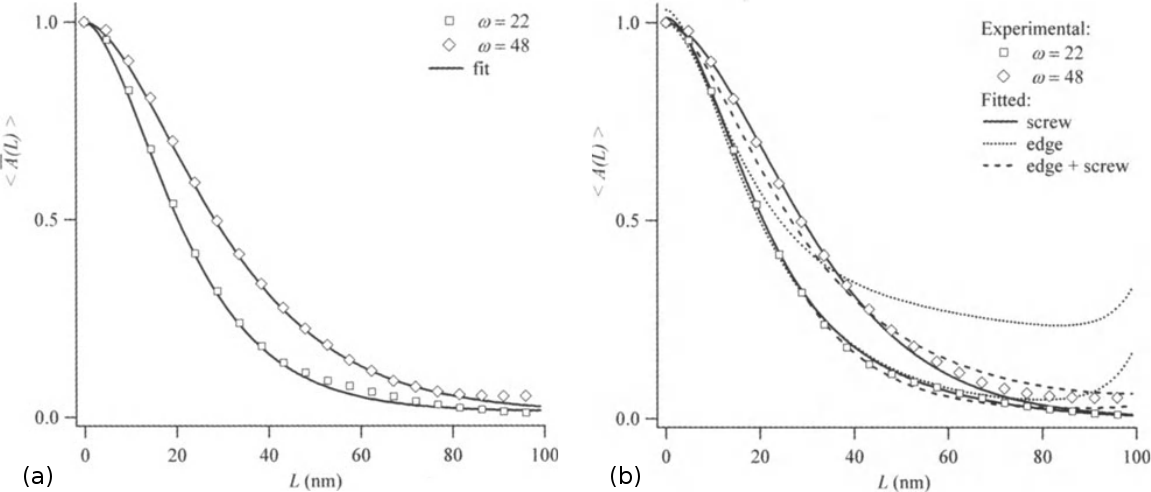
\includegraphics[width=0.8\textwidth]{Mittemeijer}
  \caption{(a) Ajuste de los coeficientes de Fourier suponiendo que todos los sistemas de deslizamiento están igualmente poblados, y con igual proporción de dislocaciones de hélice y borde. $\rho = 3 \ 10^{14}$\,m$^{-2}$. (b) Curvas de coeficientes de Fourier. En este análisis se ajustaron diferentes modelos para las curvas de $\omega = 22^{\circ}$ y se usaron los parámetros obtenidos para simular las curvas con $\omega = 48^{\circ}$. Puede apreciarse que si se supone que las dislocaciones son sólo de borde no se obtiene un buen acuerdo entre el modelo y el experimento. Por otro lado, tanto el modelo con 100\% de dislocaciones de hélice y con mitad de dislocaciones de dislocaciones de hélice y mitad de borde parecen predecir razonablemente el comportamiento observado. Las dislocaciones obtenidas son 2.2, 2.5 y 2.3 10$^{14}$\,m$^{-2}$. Imágenes obtenidas de \cite{mittemeijer2003diffraction}.}
  \label{fig:FourierMittemeijer}
\end{figure}

A partir de un análisis cristalográfico minucioso, Kamminga et al utilizaron el modelo de los factores de contraste para calcular cómo serían los coeficientes de Fourier de los las reflexiones si la dislocaciones fueran solamente de borde, solamente de hélice y si ambas estaban presentes en igual cantidad, para luego comparar dichos coeficientes con los obtenidos experimentalmente.
Haciendo esto pudieron descartar la posibilidad de que todas las dislocaciones presentes fueran de borde, sin embargo, no pudieron distinguir concluyentemente si la dislocaciones eran de borde o si eran una mezcla de ambas.
Un problema mayor es que la densidad de dislocaciones obtenida por este método no era tan diferente a la obtenida utilizando la suposición menos probable, pero más sencilla matemáticamente, de que todos los sistemas de deslizamiento estaban igualmente poblados, con igual proporción de dislocaciones de hélice y borde.
Esto significa que aunque los métodos bottom-up tienen la ventaja de general modelos que pueden vincular directamente el modelado de la microestructura con los experimentos realizados, requieren una cantidad de suposiciones a priori sobre lo que ocurre en el material microscópicamente y los datos disponibles, aún cuando son de muy buena calidad, no siempre logran distinguir concluyentemente entre diferentes posibilidades.

En este sentido es que en este trabajo también se propone trabajar siguiendo un enfoque más sencillo incialmente, pero que permitió realizar un tipo de análisis que no es posible de realizar siguiendo el enfoque bottom-up.
Este método, propuesto por Langford et al en 1982\cite{DeKeijser1982}, consiste en ajustar el pico de cada reflexión con una función de Voigt, que es la convolución de una función Gaussiana $G$ y una función Lorentziana $L$:
\begin{equation}
  V(x, H_{G}, H_{L}) \ = \ G \otimes L \ = \ \int G(x'; H_{G}) L(x - x'; H_{L}) \ dx'
  \label{eq:Voigt}
\end{equation}
\noindent
Cada una de las funciones tiene su propio FWHM, y en el modelo de Langford se asocia el FWHM de la función Gaussiana con la deformación media de la red cristalina
\begin{equation}
  <e> \ = \ \frac{1}{2} \ \sqrt{\frac{\pi}{2\log(2)}} \ \frac{H_{G}}{4 \ \tan{\theta_B}}
  \label{eq:Gauss}
\end{equation}
\noindent
y el FWHM de la función Lorentziana se asocia con la longitud promedio de cristalita en la dirección definida por el ángulo de Bragg:
\begin{equation}
  L \ = \ \frac{2}{\pi} \ \frac{\lambda}{H_{L} \ \cos{\theta_B}}
  \label{eq:Lorentz}
\end{equation}
\noindent
Al ajustar un dado pico con una función Voigtinana dejando como parámetros de ajuste a $H_G$ y $H_L$, se puede determinar la deformación promedio y la longitud de  cristalina en la dirección perpendicular a la familia de planos $\{hkl\}$ que producen interferencia constructiva para el ángulo $\theta_B$.

El problema de utilizar la Ec. \ref{eq:Voigt} para ajustar las reflexiones es que realizar un producto de convolución es muy costoso computacionalmente, por lo que unos años después Thompson et al\cite{Thompson1987} desarollaron un método para aplicar el mismo análisis, pero utilizando la llamada función pseudo-Voigt, que es una combinación lineal de una función Gaussiana y una función Lorentziana que poseen el mismo FWHM:
\begin{equation}
  pV(x; H, \eta) \ = \ \eta \ L(x; H) \ + \ (1 - \eta) \ G(x; H)
  \label{eq:pseudovoigt}
\end{equation}
\noindent
El parámetro $\eta \ \in \ [0,1]$ se denomina parámetro de mezcla e indica que tan intenso va a ser el carácter Lorentziano del pico estudiado. Al ajustar la expresión \ref{eq:pseudovoigt} e dejan como párametros de ajuste al par $[H, \eta]$ y se emplea las expresiones desarrolladas por Thompson para determinar los valores $[H_G, H_L]$ que se hubieran obtenido de realizar el ajuste utilizando la Ec. \ref{eq:Voigt}:
\begin{eqnarray}
  H_G & = & H \ (1 -  0.74417 \ \eta - 0.24781 \ \eta^2 - 0.00810 \ \eta^3)^{1/2} \\
  H_L & = & H \ (0.72928 \ \eta + 0.19289 \ \eta^2 + 0.07783 \ \eta^3)
  \label{eq:Hg}
\end{eqnarray}
\noindent
Como tanto la función Voigt como la pseudo-Voigt están normalizadas, esto es $\int V dx \ = \ \int pV dx \ = \ 1$, y para cada pico están centradas en $\theta_B$ la función que se ajusta en la práctica tiene dos parámetros libres más:
\begin{equation}
    pV(\theta; I_0, \theta_B, H, \eta) \ = \ I_0 \ [\eta \ L(\theta; \theta_B, H) \ + \ (1 - \eta) \ G(\theta; \theta_B, H)]
  \label{eq:pVprofile}
\end{equation}
\noindent
lo que permite incorporar la intensidad integrada del pico $I_0$ y el centro $\theta_B$ del mismo, y el ajuste se realiza sobre la variable angular $\theta$.

 \section{Difracción de electrones retrodifundidos}\label{S:EBSD}
La difracción de electrones retro difundidos (EBSD por sus siglas en inglés) es una técnica que se utiliza en conjunto con las técnicas de microscopía de barrido, por lo que permite no sólo caracterizar la microestructura de un material, sino correlacionar espacialmente información como la textura, tamaño de grano y acumulación de defectos.
El uso de esta técnica ha aumentado rápidamente desde principios del 2000 debido al aumento de disponibilidad de los microscopios electrónicos de barrido (SEM). El incremento de la velocidad de adquisición y procesamiento de datos también ha permitido lograr que una técnica extremadamente local (capaz de estudiar pocos cristales) pase a tener una estadística comparable, aunque aún menor, que la de los experimentos de rayos X.
\nomenclature{EBSD}{Difracción de electrones retro difundidos}
\nomenclature{SEM}{Microscopio electrónico de barrido}

Los patrones que se obtienen en una medición de EBSD se obtienen a partir de las imágenes obtenidas en una pantalla de fósforo. Un haz de electrones de alta energía incide sobre una dada muestra, e interactúa con un volumen del orden de los 20\,nm, como se muestra esquemáticamente en la Fig. \ref{fig:ebsd}.

\begin{figure}[!htb]
  \centering
  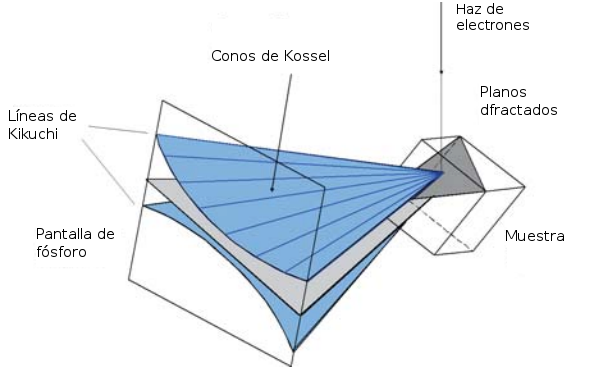
\includegraphics[width=0.6\textwidth]{ebsd.png}
  \caption{Esquema de una medición de EBSD}
  \label{fig:ebsd}
\end{figure}

Entre la multitud de interacciones que ocurren entre los electrones y el cristal, la interacción quasi elástica entre los electrones y el arreglo de planos cristalinos del volumen de interacción es la responsable de producir las llamadas bandas de Kikuchi que pueden verse en la Fig. \ref{fig:kikuchi}.
Estas bandas, que pueden pensarse como la proyección de una dada familia de planos cristalinos en la pantalla de fósforo, están limitadas por los conos de difracción que se producen cuando los electrones interactúan con la familia de planos $\{ hkl \}$. 
Se puede demostrar que el espaciamiento angular entre los llamados conos de Kossel es igual a 2$\theta_{hkl}$, donde $\theta_{hkl}$ cumple con la ley de Bragg\cite{schwartz2010electron}:
\begin{equation}
  2 \ d_{hkl} \ \sin(\theta_{hkl}) \ = \ n \ \lambda
  \label{eq:BraggEBSD}
\end{equation}
\noindent
\begin{figure}[!htb]
  \centering
  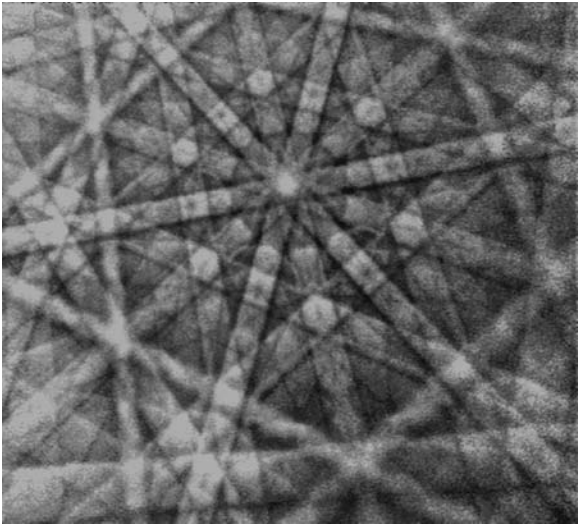
\includegraphics[width=0.6\textwidth]{kikuchi}
  \caption{Patrón de Kikuchi}
  \label{fig:kikuchi}
 \end{figure}

La configuración experimental de una medición de EBSD es tal que los conos de difracción son mucho más grandes que la pantalla de fósforo que los registra, por lo que las banda de Kikuchi que deberían ser curvas se ven practicamente rectas, lo que facilita su procesamiento y reconocimiento a través de herramientas matemáticas desarrolladas hace tiempo, en particular la transformada de Hough\cite{wiki:Hough}.

Como en la práctica el haz incidente no interactúa solamente con una familia de planos, sino con todas las familias presentes en el volumen de interacción, en la pantalla de fósforo quedan grabadas diferentes bandas de Kikuchi, cada una vinculada a una familia de planos en particular.
Como el ángulo entre las bandas de Kikuchi es igual al ángulo que tienen entre sí los diferentes planos cristalinos\cite{schwartz2010electron} se puede, si se conoce la estructura cristalina del material estudiado, determinar la orientación promedio de los cristales que interactúan con el haz de electrones.

De esta manera, en una medición de EBSD, el haz de electrones barre la muestra, y en cada ubicación registra una serie de bandas de Kikuchi a partir de las cuales determina, la orientación promedio de los cristales en el volumen estudiado.
El resultado final es una imagen en la que se registra la orientación de todos los cristales del área estudiada como la que se puede ver en la Fig. \ref{fig:ebsdex}. 
En este caso lo que se hace es asignar un color a los cristales que tienen una dada dirección cristalina paralela al eje Z y colorear cada pixel en función de este dato. 
Nótese que esta imagen, llamada mapa de figura de polo inversa, da información acerca de la dirección de los cristales y no de su orientación, aunque combinando la información de distintos mapas, toda la información orientacional de la muestra puede ser analizada.
\begin{figure}[!htb]
  \centering
  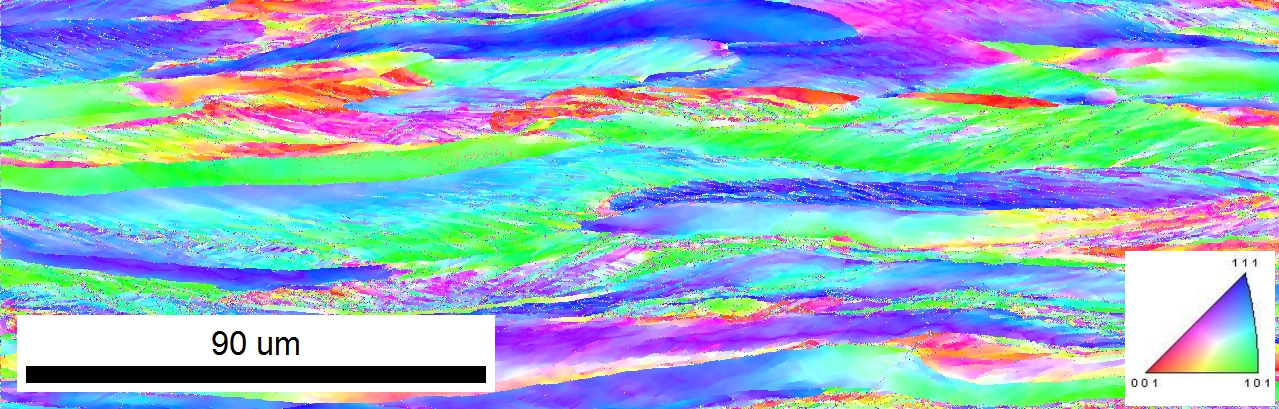
\includegraphics[width=\textwidth]{IF70centroTD-IPF}
  \caption{Ejemplo de mapa EBSD}
  \label{fig:ebsdex}
\end{figure}

Adicionalmente, los mapas de EBSD pueden proveer información acerca de la correlación espacial que existe entre las orientaciones. 
Por ejemplo, en la imagen de la Fig. \ref{fig:ebsdex} puede verse que todos los puntos que tienen direcciones similares se agrupan a lo ancho de la imagen, dando una idea de ``granos alargados'', consistente con el hecho de que la imagen mostrada proviene de una muestra laminada, con la dirección de laminación paralela a la dirección en que los granos se ``alargan''.

A partir de lo descripto anteriormente se puede apreciar que las magnitudes físicas que se pueden obtener a partir de un experimento de EBSD van a estar definidas a partir de comparar la orientación de los cristales medidos.
Por ejemplo, en un experimento de XRD uno puede estimar, a partir de las técnicas de LPA, el tamaño de los dominios coherentes de difracción, también llamados cristalitas, mientras que en EBSD se trabaja con el concepto de granos, definidos como porciones del material que tienen una misorientación mayor que determinado umbral, que suele variar entre los 5$^{\circ}$ y los 15$^{\circ}$. (escribir mejor esta parte)
Una comparación similar se puede hacer cuando se discuten las magnitudes asociadas a la deformación de la red cristalina. En los experimentos de XRD se intenta estimar la densidad de dislocaciones del material, observadas por la presencia de un ensanchamiento que crece de una manera particular con los índices  de Miller de los picos estudiados, mientras que en EBSD la cantidad básica para estimar la deformación de la red cristalina es la llama \textit{Kernel Average Misorientation} (KAM) que se define como la misorientación promedio de un pixel con sus vecinos más cercanos.
Debe quedar claro de las definiciones que tanto en las mediciones de de tamaño de grano como de deformación de la red cristalina, las magnitudes medidas a partir de XRD y de EBSD son diferentes y van a arrojar, en general, valores diferentes.
Sin embargo, es parte de las suposiciones iniciales de este trabajo que, aunque las magnitudes medidas con ambas técnicas son diferentes, su comportamiento con respecto a los procesos sometidos a los materiales debe ser qualitativamente similar, por lo que se pueden utilizar los resultados obtenidos por EBSD para constatar las conclusiones obtenidas a partir de los estudios de ancho de pico.

\section{Textura cristalográfica}\label{S:Text}
Como ya se mencionó en la Sec. \ref{S:motivacion}, las propiedades macroscópicas de un sólido cristalino estarán dadas por las propiedades de su celda unidad, y estas serán en general anisotrópicas.
Por ejemplo, si se toma un monocristal de hierro y se mide su módulo de Young $E$ en la dirección [100] se obtendrá un valor un poco inferior a los 150\,GPa, mientras que si la misma medición se realiza en la dirección [111], que forma un ángulo de unos 57$^{\circ}$ con la dirección [100], se obtendrá un valor de unos 300\,GPa, es decir, el módulo de Young se incrementará casi un 100\,\%.
Según el principio de Neumann\cite{nye1985physical} el módulo de Young de una pieza macroscópica de hierro será el promedio del módulo de Young de los diferentes cristales de Fe que se encuentren en la pieza, ponderado según la cantidad de cristales que tengan una dada orientación respecto al eje en que se aplica la tensión.
De esto se deduce que si todos los cristales está en igual proporción, el módulo de Young del hierro será isotrópico.
Para este caso particular el valor promedio es de 210\,GPa, como se puede ver en la Fig. \ref{fig:ironaniso}.

\begin{figure}[!htb]
  \centering
  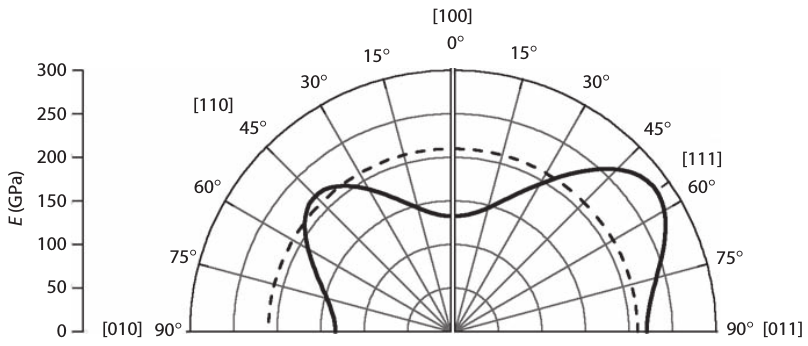
\includegraphics[width=\textwidth]{ironaniso}
  \caption{Módulo de Young $E$ para un monocristal de Hierro como función del ángulo entre la dirección [100] y el eje sobre el que se aplica la tensión. Imagen obtenida de \cite{randle2000introduction}.}
  \label{fig:ironaniso}
\end{figure}

De lo dicho anteriormente se deduce la importancia de no sólo caracterizar, sino de cuantificar la anisotropía de un material. 
En particular, se define como \textit{Textura Cristalográfica} a la orientación preferencial que tienen los diferentes cristales en un dado sólido cristalino, y la forma de estudiar cuantitaviamente la textura es la denominada \textit{Función de Distribución de Orientaciones (FDO)}.
Para poder definir adecuadamente la FDO, primero se define un sistema de referencia $K_S$ fijo a la muestra macroscópica.
La elección de $K_S$ es arbitraria, pero en general se elije de modo tal de respetar las direcciones y simetrías del material en estudio. 
Por ejemplo, para una chapa laminada, los ejes de $K_S$ suelen definirse como el de laminado (RD), el transverso (TD), que es perpendicular a RD, pero está en el plano de la chapa, y el normal (ND), perpendicular al plano RD-TD, es decir el del la chapa.
El otro sistema de referencia será solidario a un dado cristal y se lo notará $K_C$, y también elegirá de modo tal que respeta las simetrías del cristal representado.
Se define entonces a la orientación de un cristal como la rotación $\mathbf{g}$ que lleva desde el sistema de coordenadas $K_C$ al sistema $K_S$:

\begin{equation}
  K_S \ = \ \mathbf{g} \ * \ K_C
  \label{eq:orientation}
\end{equation}
\noindent

Existen muchas maneras de caracterizar a las rotaciones, pero en este trabajo se empleará fundamentalmente la de los \textit{Ángulos de Euler}, usando la convención de Bunge\cite{bunge2013texture}.
Bajo esta convención, se parte del sistema del cristal y primero se rota el mismo un ángulo $\phi_1$ alrededor del eje Z de $K_C$.
Luego se rota al nuevo sistema un ángulo $\Phi$ alrededor del nuevo eje X', y finalmente se realiza una rotación de magnitud $\phi_2$ alrededor del nuevo eje Z'', hasta que el sistema está en coincidencia con el sistema de referencia de la muestra $K_S$.
A los ángulos que constituyen la terna $\phi_1 \Phi \phi_2$ se los denomina ángulos de Euler, y son los que definen a la orientación del cristal alineado con $K_C$.
Ahora, si se tienen $N$ cristales, cada uno con una orientación $\mathbf{g}_i$ respecto al sistema de referencia de la muestra, la FDO será aquella que indique que proporción de los $N$ cristales tiene una dada orientación $\mathbf{g}$. 
En este contexto queda claro que la FDO será una función discreta, sin embargo, si el número de cristales estudiados es grande, como suele ocurrir en los experimentos de XRD, se puede definir a la FDO como una función continua $f(\mathbf{g})$ en el espacio de orientaciones.
De esta manera se tiene que la FDO es la función que determina la fracción de volumen que representan los cristales con una orientación que cae en una región $\Delta \Omega$ del espacio de orientaciones\cite{kocks2000texture}:
\begin{equation}
  \frac{\Delta V}{V} \ = \ \frac{\int_{\Delta \Omega} \ f(\mathbf{g}) \ d\mathbf{g}}{\int_{\Omega_0} \ f(\mathbf{g})\ d\mathbf{g}}
  \label{eq:ODF}
\end{equation}
\noindent
donde $\Omega_0$ es el espacio total considerado, que puede tener un volumen máximo de $8\pi^2$ o un valor menor dado por el volumen del subespacio irreducible que se obtiene de aplicar al espacio total los grupos de simetría de la red de Bravais considerada más las simetrías de muestras que pudieran existir.
Si la orientaciones se representan usando los ángulos de Euler, el elemento infinitesimal de volumen vale:
\begin{equation}
  d\mathbf{g} \ = \ \frac{1}{8\pi^2} \sin(\Phi) d\phi_1 d\Phi d\phi_2
  \label{eq:dg}
\end{equation}
\noindent
donde el factor $1/(8\pi^2)$ es un factor de normalización que se vuelve necesario si se conviene que $f(\mathbf{g}) \ \equiv \ 1$ para un material con una FDO uniforme.

\subsection{Determinación de la FDO}\label{SS:FDO}
La forma más sencilla de determinar la FDO para un dado material sería medir la orientación de cada uno de los cristales que están presentes en un cierto volumen $V$, para luego computar la FDO exacta (discreta), que luego puede aproximarse por la $f(\mathbf{g})$ continua, que es más fácil de manipular matemáticamente.
Esta tarea puede realizarse a partir de los experimentos de EBSD descriptos en la sección \ref{S:EBSD}, con el beneficio además de que se puede obtener la orientación de los cristales en función de la posición de la muestra, lo que provee una descripción en principio más completa de la microestructura del material.
Sin embargo, incluso con los avances en automatización y procesamiento de los microscopios modernos, la medición de un volumen de muestra que sea representativo del todo el material a través de los experimentos de EBSD, es una tarea difícil, y a veces posible de lograr.

Por otro lado, los volúmenes de interacción de la radiación de rayos X son muchos más grandes que los que se pueden conseguir con electrones, por lo que la medición de volumen representativo del material se vuelve mucho más sencilla, aunque los rayos X sólo pueden medir proyecciones de $f(\mathbf{g})$ llamadas figuras de polos (FP).
Para medir una FP en un experimento de XRD se selecciona una dada familia de planos $\{hkl\}$ colocando el detector a un ángulo $2\theta$ adecuado y se mide la inteensidad de dicha reflexión.
En esta situación, los únicos cristales que contribuirán a la intensidad de la reflexión medida son aquellos cuya dirección $[hkl]$ sea perpendicular a la superficie de la muestra, es decir, la intensidad de una figura de polos en una dada dirección $\mathbf{y}$ es proporcional a la cantidad de cristales que cumplen la condición $[hkl] \ // \ y$, lo que se puede expresar como una proyección de la FDO $f(\mathbf{g})$:
\begin{equation}
  p_{\mathbf{h}}(\mathbf{y}) \ = \ \int_{0}^{2\pi} \ f(\mathbf{g}) \ d\mathbf{\Gamma}
  \label{eq:PDF}
\end{equation}
\noindent
donde $\mathbf{h} \ = \ [hkl]$ y $\Gamma$ es un cierto camino dentro del espacio de orientaciones que se obtiene al efectuar una rotación completa alrededor del polo $[hkl]$.

Para resolver el problema de inversión de las figuras de polos, es decir, para obener $f(\mathbf{g})$ a partir de la medición de diferentes $p_{\mathbf{h}}(\mathbf{y})$, Bunge partió del hecho que $f(\mathbf{g})$ puede desarrollarse en armónicos esféricos:
\begin{equation}
  f(\mathbf{g}) \ = \ \sum_{l=0}^{\infty} \sum_{\mu=1}^{M(l)} \sum_{\nu=1}^{N(l)} C_{l}^{\mu \nu} \ T_{l}^{\mu \nu}(\mathbf{g})
  \label{eq:ODFharm}
\end{equation}
\noindent
donde $C_{l}^{\mu \nu}$ son los coeficientes del desarrollo de $f(\mathbf{g}$ y $T_{l}^{\mu \nu}(\mathbf{g})$ son los armónicos esféricos generalizados.
Por otro lado, al ser una proyección, para cada $\mathbf{h}_i$, $p_{\mathbf{h}}(\mathbf{y})$ se puede desarrollar en armónicos esféricos superficiales:
\begin{equation}
  p_{\mathbf{h}_i}(\mathbf{y}) \ = \ \sum_{l=0}^{\infty} \sum_{\nu=1}^{N(l)} F_{l}^{\nu}(\mathbf{h}_i) \ k_{l}^{\nu}(\mathbf{y}
  \label{eq:PDFharm}
\end{equation}
\noindent
con
\begin{equation}
  F_{l}^{\nu}(\mathbf{h}_i) \ = \ \frac{4 \pi}{2l + 1} \sum_{\mu=1}^{M(l)} C_{l}^{\mu \nu} \ k_{l}^{* \mu}(\mathbf{h}_i)
  \label{eq:FPDFharm}
\end{equation}
\noindent
A partir de combinar las Ecs. \ref{eq:PDF}, \ref{eq:ODFharm} y \ref{eq:PDFharm}, realizar varias integrales e igualar coeficientes, Bunge llegó a la relación que permite determinar los coeficientes $C_{l}^{\mu \nu}$ a partir de las FP experimentales\cite{bunge2013texture}:
\begin{equation}
  F_{l}^{\nu}(\mathbf{h}_i) \ = \ 4 \pi \frac{\oint \ p_{\mathbf{h}_i}(\mathbf{y}) \ k_{l}^{* \nu} \ d\mathbf{\Gamma}}{\oint \ p_{\mathbf{h}_i}(\mathbf{y}) \ d\mathbf{\Gamma}}
  \label{eq:CoefHarm}
\end{equation}
\noindent
La Ec. \ref{eq:CoefHarm} permite entonces la determinación experimental de los coeficientes $F_{l}^{\nu}(\mathbf{h}_i)$, que junto con la igualdad \ref{eq:FPDFharm} constituyen un sistema de $i$ ecuaciones (una por cada FP medida) e infinitas incógnitas, de donde se deduce que para determinar completamente una FDO se necesecitan medir infinitas FPs, lo cual es imposible en la práctica.
No obstante este problema, Bunge\cite{bunge2013texture} también logró demostrar que dependiendo de la simetrías de cristal y de muestra dadas, el número de coeficientes independientes en \ref{eq:FPDFharm} se puede reducir notablemente, cómo se pude ver en la Fig. \ref{fig:harmonics}, lo que permite estimar la FDO con una precisión razonable habiendo medido sólo unas pocas FPs, ya que el empleo de las simetrías permite conocer coeficientes de órdenes más altos a partir de aquellos de órdenes más bajos. 
Por ejemplo para materiales con simetría cristalina cúbica, se puede recostruir razonablemente bien la FDO solamente con tres FPs.
\begin{figure}[!htb]
  \centering
  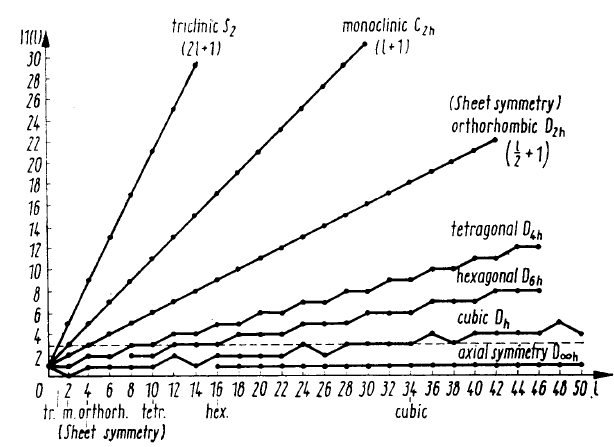
\includegraphics[width=0.7\textwidth]{harmonics}
  \caption{Cantidad de coefcientes independientes en un desarrollo de armónicos esféricos como función del grado $l$. La línea de puntos en la figura indica el máximo orden del desarrollo en armónicos esféricos de la Función de Distribución de Orientaciones que se puede obtener habiendo medido tres Figuras de Polos.}
  \label{fig:harmonics}
\end{figure}

Otra cantidad que se puede derivar a partir de $f(\mathbf{g})$ es la llamada \textit{Figura de Polos Inversa (FPI)} que se obtiene de contar cuántos cristales tienen una cierta familia de planos $\mathbf{h}$ en la dirección $\mathbf{y}$ de la muestra, lo que matemáticamente se expresa como
\begin{equation}
  a_{\mathbf{y}}(\mathbf{h}) \ = \ \frac{1}{2 \pi} \oint f(\mathbf{g}) d\Gamma
  \label{eq:IPF}
\end{equation}
\noindent
Sobre qué camino se integra?

Describo el método de MTEX?
% \subsection{La textura, su relación con la microestructura y los procesos de deformación}\label{SS:Defo}
\subsection{FDO y FDO generalizada}\label{SS:ODFG}
Según lo explicado en la Sec. \ref{S:DRX}, la determinación de la FDO se puede hacer a partir de la medición de figuras de polos, que a su vez pueden ser determinadas por medio de experimentos de XRD, ya que en dichos experimentos se tiene que la intensidad integrada de la reflexión $\{hkl\}$ es proporcional al número de planos cristalinos paralelos a  la superficie del material en la dirección $\mathbf{y}$.
Ahora bien, como ya se discutió previamente, a partir del estudio de la forma de picos medidos en la misma dirección $\mathbf{y}$ se puede determinar el tamaño de la microestructura de los planos $\{hkl\}$ que pertenecen a los cristales que están difractando.
Por ejemplo, si me mide completamente el pico de la reflexión $hkl$ se puede determinar la proporción de cristales que tienen sus planos $\{hkl\}$ paralelos a la superficie del material, pero además se puede a partir del ancho $H$ de dicho pico estimar la longitud de la columna que difracta coherentemente en la dirección $[hkl]$ empleando la Ec. [poner ec de tamaño de Langford] y ver la distorsión perpendicular a esa dirección utilizando la Ec. [poner ec de strain en Langford].
De esta manera se puede asignar a la dirección $\mathbf{y}$ no sólo un número asociado al número de cristales con sus planos en esa dirección, sino un par de números que indicarán el estado de la microestructura de los planos cristalinos orientados en dicha dirección, lo que permite construir lo que se denominas \textit{Figuras de Polos Generalizadas (FPG)} de tamaño de dominio o de distorsión, respectivamente.

Es más, si se incorpora la suposición \textit{ad-hoc} de que el ensanchamiento de los picos es proporcional a la energía acumulada en dichos cristales se pueden extender heurísticamente los procedimientos explicados en la Sec. \ref{S:Text} para estimar las FDO a partir de las FP, y utilizarlos para calcular una \textit{Función de Distribución de Orientaciones Generalizada (FDOG)} a partir de las FPG. 
De esta manera, a partir de un análisis integral de las FDO y las FDOG se puede, en principio estudiar no sólo la orientación preferencial de los cristales para un dado proceso de deformación, sino hacer un análisis semicuantitativo de cómo es la microestructura de los cristales que tienen orienciones similares, lo cual permite extraer muchas conclusiones acerca de como es la anisotropía en la la acumulación de defectos para un determinado material en alguna situación de interés. 
% \section{Revisión bibliográfica y estado del arte}\label{S:RB}

\section{Organización de la tesis}\label{S:Org}
En el Cap. \ref{C:Materiales} se explicarán lo detalles de los experimentos de difracción de rayos X que se realizaron para ponder medir la texura de los materiales estudiados en el desarrollo de esta tesis. 
También se explicarán los algoritmos empleados para poder procesar el gran caudal de datos que se obtiene de un experimento de XRD realizado con luz sincrotrón, así como una descripción del método empleado en las mediciones de EBSD que usaron para corroborar los resultados obtenidos por medio de las técnicas de LPA aplicada a los resultados de sincrotrón.

Cada uno de los capítulos que siguen de la Sec. \ref{C:Materiales} está dedicado a uno de los materiales estudiados.
En los capítulos \ref{C:IF}, \ref{C:F138} y \ref{C:G2205} se estudian tres aceros con caracterísitcas diferentes: el del Cap. \ref{C:IF} es un acero denominado libre de intersticiales (IF) que tiene una estructura cristalina de tipo BCC, el del Cap. \ref{C:F138} es un acero inoxidable denominado F138, que tiene un estructura de tipo FCC y también se estudió un acero de dos fases (BCC + FCC) nomenclado G2205, y cuyos principales resultados se encuentran en el Cap. \ref{C:G2205}.

En el Cap. \ref{C:Al} se muestran los resultados de aplicar los métodos descriptos en un aluminio 1050 obtenido comericialmente.
Al final de cada capítulo se encuentra una conclusión particular que considera lo visto con cada material individualmente, y en el Cap. \ref{C:Conclusiones} se presenta una conclusión general del trabajo.

Finalmente en el Cap. \ref{C:Proyecciones} pueden apreciarse posibles caminos a seguir a partir de los resultados obtenidos en esta tesis.
